\documentclass[border=8pt]{standalone}
\usepackage{tikz}
\usetikzlibrary{positioning,arrows.meta,shapes.geometric,fit,backgrounds,calc}
\usepackage[T1]{fontenc}
\usepackage{helvet}
\renewcommand{\familydefault}{\sfdefault}

\definecolor{inputblue}{HTML}{3B82F6}
\definecolor{processgreen}{HTML}{10B981}
\definecolor{modelviolet}{HTML}{8B5CF6}
\definecolor{dashorange}{HTML}{F59E0B}
\definecolor{storered}{HTML}{EF4444}
\definecolor{bgdark}{HTML}{1E293B}
\definecolor{boxbg}{HTML}{334155}

\begin{document}
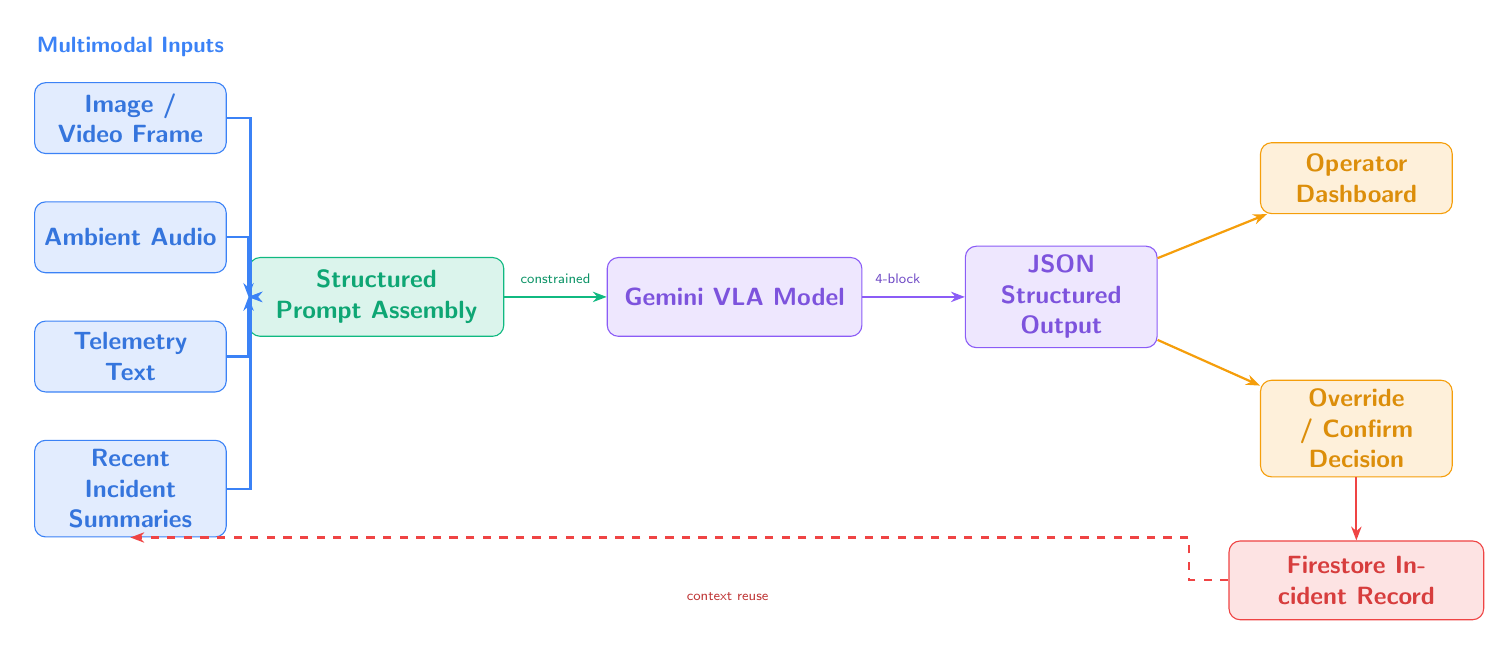
\begin{tikzpicture}[
    node distance=0.6cm and 1.0cm,
    every node/.style={font=\small},
    block/.style={rectangle, rounded corners=4pt, draw=#1, fill=#1!15, 
                  text width=2.2cm, minimum height=0.9cm, align=center,
                  font=\small\bfseries, text=#1!90!black},
    bigblock/.style={rectangle, rounded corners=4pt, draw=#1, fill=#1!15,
                     text width=3.0cm, minimum height=1.0cm, align=center,
                     font=\small\bfseries, text=#1!90!black},
    arrow/.style={-{Stealth[length=5pt]}, thick, color=#1},
    grouplabel/.style={font=\footnotesize\bfseries, text=#1},
]

% Input Layer
\node[block=inputblue] (image) {Image / Video Frame};
\node[block=inputblue, below=of image] (audio) {Ambient Audio};
\node[block=inputblue, below=of audio] (telem) {Telemetry Text};
\node[block=inputblue, below=of telem] (history) {Recent Incident Summaries};

% Group label
\node[grouplabel=inputblue, above=0.2cm of image] {\textsc{Multimodal Inputs}};

% Processing
\node[bigblock=processgreen, right=1.5cm of $(audio)!0.5!(telem)$] (prompt) {Structured Prompt Assembly};

% Model
\node[bigblock=modelviolet, right=1.3cm of prompt] (gemini) {Gemini VLA Model};

% Output
\node[block=modelviolet, right=1.3cm of gemini] (json) {JSON Structured Output};

% Dashboard
\node[block=dashorange, above right=0.4cm and 1.3cm of json] (dashboard) {Operator Dashboard};
\node[block=dashorange, below right=0.4cm and 1.3cm of json] (override) {Override / Confirm Decision};

% Storage
\node[bigblock=storered, below=0.8cm of override] (firestore) {Firestore Incident Record};

% Arrows - inputs to prompt
\draw[arrow=inputblue] (image.east) -- ++(0.3,0) |- (prompt.west);
\draw[arrow=inputblue] (audio.east) -- (audio.east -| prompt.west) -- (prompt.west);
\draw[arrow=inputblue] (telem.east) -- (telem.east -| prompt.west) -- (prompt.west);
\draw[arrow=inputblue] (history.east) -- ++(0.3,0) |- (prompt.west);

% Prompt to model
\draw[arrow=processgreen] (prompt) -- (gemini);

% Model to JSON
\draw[arrow=modelviolet] (gemini) -- (json);

% JSON to dashboard
\draw[arrow=dashorange] (json) -- (dashboard);
\draw[arrow=dashorange] (json) -- (override);

% Override to storage
\draw[arrow=storered] (override) -- (firestore);

% Feedback loop: storage back to history
\draw[arrow=storered, dashed] (firestore.west) -- ++(-0.5,0) |- (history.south);

% Labels on arrows
\node[font=\tiny, text=processgreen!80!black, above=0.05cm] at ($(prompt)!0.5!(gemini)$) {constrained};
\node[font=\tiny, text=modelviolet!80!black, above=0.05cm] at ($(gemini)!0.5!(json)$) {4-block};
\node[font=\tiny, text=storered!80!black, below left=0.05cm and 0cm, anchor=north] at ($(firestore.south west)!0.5!(history.south east)$) {context reuse};

\end{tikzpicture}
\end{document}
